% Created by tikzDevice version 0.7.0 on 2016-08-15 15:02:32
% !TEX encoding = UTF-8 Unicode
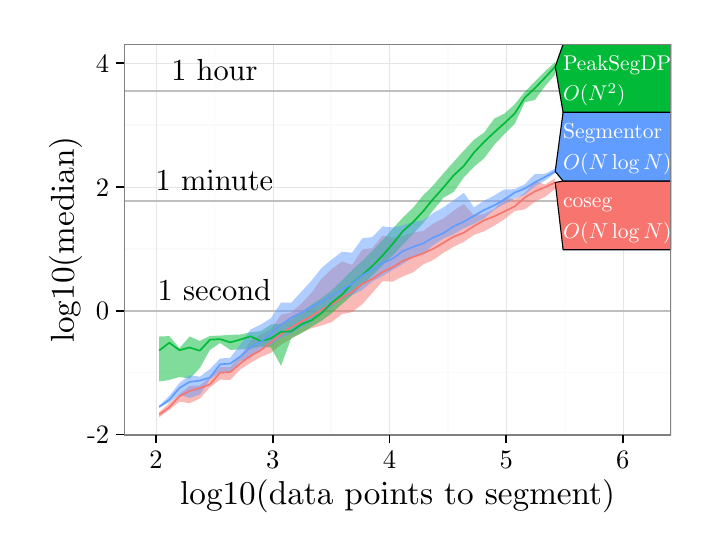
\begin{tikzpicture}[x=1pt,y=1pt]
\definecolor[named]{fillColor}{rgb}{1.00,1.00,1.00}
\path[use as bounding box,fill=fillColor,fill opacity=0.00] (0,0) rectangle (238.49,180.67);
\begin{scope}
\path[clip] (  0.00,  0.00) rectangle (238.49,180.67);
\definecolor[named]{drawColor}{rgb}{1.00,1.00,1.00}
\definecolor[named]{fillColor}{rgb}{1.00,1.00,1.00}

\path[draw=drawColor,line width= 0.6pt,line join=round,line cap=round,fill=fillColor] (  0.00,  0.00) rectangle (238.49,180.68);
\end{scope}
\begin{scope}
\path[clip] ( 34.86, 33.48) rectangle (232.49,174.67);
\definecolor[named]{fillColor}{rgb}{1.00,1.00,1.00}

\path[fill=fillColor] ( 34.86, 33.48) rectangle (232.49,174.67);
\definecolor[named]{drawColor}{rgb}{0.98,0.98,0.98}

\path[draw=drawColor,line width= 0.6pt,line join=round] ( 34.86, 56.02) --
	(232.49, 56.02);

\path[draw=drawColor,line width= 0.6pt,line join=round] ( 34.86,100.74) --
	(232.49,100.74);

\path[draw=drawColor,line width= 0.6pt,line join=round] ( 34.86,145.46) --
	(232.49,145.46);

\path[draw=drawColor,line width= 0.6pt,line join=round] ( 67.48, 33.48) --
	( 67.48,174.67);

\path[draw=drawColor,line width= 0.6pt,line join=round] (109.65, 33.48) --
	(109.65,174.67);

\path[draw=drawColor,line width= 0.6pt,line join=round] (151.82, 33.48) --
	(151.82,174.67);

\path[draw=drawColor,line width= 0.6pt,line join=round] (193.99, 33.48) --
	(193.99,174.67);
\definecolor[named]{drawColor}{rgb}{0.90,0.90,0.90}

\path[draw=drawColor,line width= 0.2pt,line join=round] ( 34.86, 33.66) --
	(232.49, 33.66);

\path[draw=drawColor,line width= 0.2pt,line join=round] ( 34.86, 78.38) --
	(232.49, 78.38);

\path[draw=drawColor,line width= 0.2pt,line join=round] ( 34.86,123.10) --
	(232.49,123.10);

\path[draw=drawColor,line width= 0.2pt,line join=round] ( 34.86,167.81) --
	(232.49,167.81);

\path[draw=drawColor,line width= 0.2pt,line join=round] ( 46.40, 33.48) --
	( 46.40,174.67);

\path[draw=drawColor,line width= 0.2pt,line join=round] ( 88.57, 33.48) --
	( 88.57,174.67);

\path[draw=drawColor,line width= 0.2pt,line join=round] (130.74, 33.48) --
	(130.74,174.67);

\path[draw=drawColor,line width= 0.2pt,line join=round] (172.90, 33.48) --
	(172.90,174.67);

\path[draw=drawColor,line width= 0.2pt,line join=round] (215.07, 33.48) --
	(215.07,174.67);
\definecolor[named]{drawColor}{rgb}{0.75,0.75,0.75}
\definecolor[named]{fillColor}{rgb}{0.75,0.75,0.75}

\path[draw=drawColor,line width= 0.6pt,line join=round,fill=fillColor] ( 34.86, 78.38) -- (232.49, 78.38);

\path[draw=drawColor,line width= 0.6pt,line join=round,fill=fillColor] ( 34.86,118.14) -- (232.49,118.14);

\path[draw=drawColor,line width= 0.6pt,line join=round,fill=fillColor] ( 34.86,157.89) -- (232.49,157.89);
\definecolor[named]{fillColor}{rgb}{0.97,0.46,0.43}

\path[fill=fillColor,fill opacity=0.50] ( 47.52, 41.75) --
	( 51.18, 44.96) --
	( 54.85, 48.27) --
	( 58.52, 51.22) --
	( 62.19, 51.38) --
	( 65.86, 54.33) --
	( 69.53, 58.03) --
	( 73.20, 58.03) --
	( 76.87, 62.05) --
	( 80.54, 67.50) --
	( 84.21, 69.75) --
	( 87.88, 71.67) --
	( 91.55, 76.97) --
	( 95.22, 77.72) --
	( 98.89, 80.98) --
	(102.56, 84.85) --
	(106.23, 89.99) --
	(109.90, 93.44) --
	(113.57, 96.18) --
	(117.24, 94.96) --
	(120.91,100.47) --
	(124.57,101.04) --
	(128.24,105.52) --
	(131.91,104.84) --
	(135.58,105.37) --
	(139.25,106.66) --
	(142.92,107.20) --
	(146.59,109.91) --
	(150.26,111.72) --
	(153.93,114.58) --
	(157.60,116.98) --
	(161.27,112.75) --
	(164.94,113.33) --
	(168.61,115.17) --
	(172.28,119.26) --
	(175.95,118.62) --
	(179.62,120.85) --
	(183.29,125.29) --
	(186.96,124.01) --
	(190.63,126.28) --
	(190.63,122.39) --
	(186.96,119.52) --
	(183.29,117.74) --
	(179.62,115.01) --
	(175.95,114.40) --
	(172.28,111.47) --
	(168.61,109.13) --
	(164.94,107.10) --
	(161.27,105.79) --
	(157.60,103.26) --
	(153.93,101.53) --
	(150.26, 99.34) --
	(146.59, 96.78) --
	(142.92, 95.11) --
	(139.25, 92.25) --
	(135.58, 90.82) --
	(131.91, 88.90) --
	(128.24, 89.08) --
	(124.57, 84.85) --
	(120.91, 80.73) --
	(117.24, 77.89) --
	(113.57, 77.18) --
	(109.90, 74.30) --
	(106.23, 73.06) --
	(102.56, 72.05) --
	( 98.89, 70.43) --
	( 95.22, 68.24) --
	( 91.55, 66.12) --
	( 87.88, 63.18) --
	( 84.21, 61.62) --
	( 80.54, 59.56) --
	( 76.87, 57.21) --
	( 73.20, 53.36) --
	( 69.53, 53.48) --
	( 65.86, 50.73) --
	( 62.19, 46.63) --
	( 58.52, 44.96) --
	( 54.85, 45.55) --
	( 51.18, 42.56) --
	( 47.52, 39.89) --
	cycle;
\definecolor[named]{fillColor}{rgb}{0.00,0.73,0.22}

\path[fill=fillColor,fill opacity=0.50] ( 47.52, 69.06) --
	( 51.18, 69.21) --
	( 54.85, 64.88) --
	( 58.52, 69.09) --
	( 62.19, 67.47) --
	( 65.86, 69.26) --
	( 69.53, 69.41) --
	( 73.20, 69.67) --
	( 76.87, 69.77) --
	( 80.54, 70.63) --
	( 84.21, 70.99) --
	( 87.88, 73.39) --
	( 91.55, 73.67) --
	( 95.22, 75.20) --
	( 98.89, 77.82) --
	(102.56, 80.59) --
	(106.23, 82.94) --
	(109.90, 85.77) --
	(113.57, 89.38) --
	(117.24, 93.04) --
	(120.91, 96.45) --
	(124.57,100.05) --
	(128.24,103.82) --
	(131.91,108.06) --
	(135.58,112.05) --
	(139.25,115.58) --
	(142.92,120.10) --
	(146.59,123.74) --
	(150.26,128.05) --
	(153.93,132.18) --
	(157.60,136.25) --
	(161.27,140.19) --
	(164.94,142.77) --
	(168.61,147.82) --
	(172.28,149.62) --
	(175.95,152.94) --
	(179.62,157.48) --
	(183.29,161.24) --
	(186.96,164.94) --
	(190.63,168.26) --
	(190.63,163.71) --
	(186.96,159.54) --
	(183.29,154.55) --
	(179.62,153.71) --
	(175.95,145.85) --
	(172.28,142.19) --
	(168.61,138.37) --
	(164.94,133.45) --
	(161.27,130.38) --
	(157.60,126.58) --
	(153.93,121.29) --
	(150.26,119.22) --
	(146.59,114.75) --
	(142.92,110.04) --
	(139.25,106.16) --
	(135.58,102.31) --
	(131.91, 98.42) --
	(128.24, 94.79) --
	(124.57, 91.19) --
	(120.91, 87.71) --
	(117.24, 84.03) --
	(113.57, 80.78) --
	(109.90, 77.50) --
	(106.23, 74.80) --
	(102.56, 72.57) --
	( 98.89, 70.25) --
	( 95.22, 68.46) --
	( 91.55, 58.49) --
	( 87.88, 65.11) --
	( 84.21, 65.48) --
	( 80.54, 64.68) --
	( 76.87, 64.40) --
	( 73.20, 64.23) --
	( 69.53, 66.69) --
	( 65.86, 64.23) --
	( 62.19, 57.63) --
	( 58.52, 53.85) --
	( 54.85, 54.44) --
	( 51.18, 53.36) --
	( 47.52, 52.83) --
	cycle;
\definecolor[named]{fillColor}{rgb}{0.38,0.61,1.00}

\path[fill=fillColor,fill opacity=0.50] ( 47.52, 44.00) --
	( 51.18, 47.60) --
	( 54.85, 52.28) --
	( 58.52, 55.10) --
	( 62.19, 54.56) --
	( 65.86, 57.29) --
	( 69.53, 61.12) --
	( 73.20, 61.40) --
	( 76.87, 66.19) --
	( 80.54, 71.61) --
	( 84.21, 73.39) --
	( 87.88, 75.66) --
	( 91.55, 81.34) --
	( 95.22, 81.25) --
	( 98.89, 85.29) --
	(102.56, 89.29) --
	(106.23, 93.87) --
	(109.90, 96.92) --
	(113.57, 99.71) --
	(117.24, 99.35) --
	(120.91,104.51) --
	(124.57,105.01) --
	(128.24,108.86) --
	(131.91,108.48) --
	(135.58,109.24) --
	(139.25,110.47) --
	(142.92,111.07) --
	(146.59,113.71) --
	(150.26,115.75) --
	(153.93,118.30) --
	(157.60,121.01) --
	(161.27,115.74) --
	(164.94,118.17) --
	(168.61,120.04) --
	(172.28,122.26) --
	(175.95,122.29) --
	(179.62,124.07) --
	(183.29,127.84) --
	(186.96,127.86) --
	(190.63,129.76) --
	(190.63,128.12) --
	(186.96,125.40) --
	(183.29,123.34) --
	(179.62,120.27) --
	(175.95,118.95) --
	(172.28,116.97) --
	(168.61,114.86) --
	(164.94,111.79) --
	(161.27,109.82) --
	(157.60,108.16) --
	(153.93,106.03) --
	(150.26,104.48) --
	(146.59,102.09) --
	(142.92, 98.90) --
	(139.25, 97.76) --
	(135.58, 95.25) --
	(131.91, 93.15) --
	(128.24, 90.91) --
	(124.57, 89.00) --
	(120.91, 85.89) --
	(117.24, 84.09) --
	(113.57, 82.55) --
	(109.90, 79.55) --
	(106.23, 77.59) --
	(102.56, 74.27) --
	( 98.89, 72.36) --
	( 95.22, 70.18) --
	( 91.55, 68.51) --
	( 87.88, 65.88) --
	( 84.21, 64.56) --
	( 80.54, 61.40) --
	( 76.87, 60.21) --
	( 73.20, 56.21) --
	( 69.53, 56.31) --
	( 65.86, 53.61) --
	( 62.19, 48.05) --
	( 58.52, 46.88) --
	( 54.85, 48.05) --
	( 51.18, 45.26) --
	( 47.52, 43.31) --
	cycle;
\definecolor[named]{drawColor}{rgb}{0.97,0.46,0.43}

\path[draw=drawColor,line width= 0.6pt,line join=round] ( 47.52, 40.87) --
	( 51.18, 43.48) --
	( 54.85, 47.48) --
	( 58.52, 49.39) --
	( 62.19, 50.39) --
	( 65.86, 51.76) --
	( 69.53, 56.02) --
	( 73.20, 56.21) --
	( 76.87, 59.36) --
	( 80.54, 62.10) --
	( 84.21, 64.09) --
	( 87.88, 66.94) --
	( 91.55, 69.91) --
	( 95.22, 72.43) --
	( 98.89, 74.48) --
	(102.56, 76.42) --
	(106.23, 78.75) --
	(109.90, 80.73) --
	(113.57, 83.09) --
	(117.24, 85.14) --
	(120.91, 88.10) --
	(124.57, 89.86) --
	(128.24, 92.39) --
	(131.91, 94.08) --
	(135.58, 96.39) --
	(139.25, 97.79) --
	(142.92, 99.12) --
	(146.59,100.79) --
	(150.26,102.96) --
	(153.93,105.16) --
	(157.60,106.58) --
	(161.27,108.99) --
	(164.94,111.08) --
	(168.61,112.49) --
	(172.28,114.29) --
	(175.95,116.05) --
	(179.62,119.25) --
	(183.29,121.52) --
	(186.96,123.02) --
	(190.63,124.72);
\definecolor[named]{drawColor}{rgb}{0.00,0.73,0.22}

\path[draw=drawColor,line width= 0.6pt,line join=round] ( 47.52, 64.00) --
	( 51.18, 66.83) --
	( 54.85, 64.11) --
	( 58.52, 65.11) --
	( 62.19, 63.94) --
	( 65.86, 67.90) --
	( 69.53, 68.14) --
	( 73.20, 66.94) --
	( 76.87, 67.99) --
	( 80.54, 69.14) --
	( 84.21, 67.39) --
	( 87.88, 68.38) --
	( 91.55, 70.78) --
	( 95.22, 70.89) --
	( 98.89, 73.50) --
	(102.56, 74.93) --
	(106.23, 77.59) --
	(109.90, 81.30) --
	(113.57, 84.17) --
	(117.24, 88.30) --
	(120.91, 91.24) --
	(124.57, 94.61) --
	(128.24, 98.31) --
	(131.91,102.56) --
	(135.58,107.14) --
	(139.25,110.39) --
	(142.92,114.34) --
	(146.59,118.84) --
	(150.26,122.92) --
	(153.93,127.31) --
	(157.60,130.71) --
	(161.27,135.54) --
	(164.94,139.39) --
	(168.61,142.87) --
	(172.28,146.16) --
	(175.95,149.60) --
	(179.62,155.37) --
	(183.29,158.82) --
	(186.96,162.65) --
	(190.63,166.59);
\definecolor[named]{drawColor}{rgb}{0.38,0.61,1.00}

\path[draw=drawColor,line width= 0.6pt,line join=round] ( 47.52, 43.66) --
	( 51.18, 46.23) --
	( 54.85, 50.48) --
	( 58.52, 52.70) --
	( 62.19, 53.10) --
	( 65.86, 54.27) --
	( 69.53, 59.01) --
	( 73.20, 59.29) --
	( 76.87, 61.84) --
	( 80.54, 65.19) --
	( 84.21, 67.12) --
	( 87.88, 70.06) --
	( 91.55, 73.29) --
	( 95.22, 75.84) --
	( 98.89, 77.70) --
	(102.56, 79.75) --
	(106.23, 81.55) --
	(109.90, 83.78) --
	(113.57, 86.07) --
	(117.24, 88.11) --
	(120.91, 91.09) --
	(124.57, 93.32) --
	(128.24, 95.55) --
	(131.91, 97.24) --
	(135.58, 99.93) --
	(139.25,101.45) --
	(142.92,102.71) --
	(146.59,104.86) --
	(150.26,106.42) --
	(153.93,108.86) --
	(157.60,110.53) --
	(161.27,112.68) --
	(164.94,114.80) --
	(168.61,116.45) --
	(172.28,118.61) --
	(175.95,121.09) --
	(179.62,122.53) --
	(183.29,124.79) --
	(186.96,126.72) --
	(190.63,128.73);
\definecolor[named]{drawColor}{rgb}{0.00,0.00,0.00}

\node[text=drawColor,anchor=base,inner sep=0pt, outer sep=0pt, scale=  1.10] at ( 67.48, 82.18) {1 second};

\node[text=drawColor,anchor=base,inner sep=0pt, outer sep=0pt, scale=  1.10] at ( 67.48,121.94) {1 minute};

\node[text=drawColor,anchor=base,inner sep=0pt, outer sep=0pt, scale=  1.10] at ( 67.48,161.70) {1 hour};
\end{scope}
\begin{scope}
\path[clip] ( 34.86, 33.48) rectangle (232.49,174.67);
\definecolor[named]{drawColor}{rgb}{0.00,0.00,0.00}
\definecolor[named]{fillColor}{rgb}{0.97,0.46,0.43}

\path[draw=drawColor,line width= 0.4pt,line join=round,line cap=round,fill=fillColor] (190.63,124.72) --
	(193.47,125.26) --
	(232.49,125.26) --
	(232.49,100.44) --
	(193.47,100.44) --
	cycle;
\definecolor[named]{fillColor}{rgb}{0.38,0.61,1.00}

\path[draw=drawColor,line width= 0.4pt,line join=round,line cap=round,fill=fillColor] (190.63,128.73) --
	(193.47,150.09) --
	(232.49,150.09) --
	(232.49,125.26) --
	(193.47,125.26) --
	cycle;
\definecolor[named]{fillColor}{rgb}{0.00,0.73,0.22}

\path[draw=drawColor,line width= 0.4pt,line join=round,line cap=round,fill=fillColor] (190.63,166.59) --
	(193.47,174.67) --
	(232.49,174.67) --
	(232.49,150.09) --
	(193.47,150.09) --
	cycle;
\definecolor[named]{drawColor}{rgb}{1.00,1.00,1.00}

\node[text=drawColor,anchor=base west,inner sep=0pt, outer sep=0pt, scale=  0.78] at (193.47,115.77) {coseg};

\node[text=drawColor,anchor=base west,inner sep=0pt, outer sep=0pt, scale=  0.78] at (193.47,104.57) {$O(N \log N)$};

\node[text=drawColor,anchor=base west,inner sep=0pt, outer sep=0pt, scale=  0.78] at (193.47,140.60) {Segmentor};

\node[text=drawColor,anchor=base west,inner sep=0pt, outer sep=0pt, scale=  0.78] at (193.47,129.40) {$O(N \log N)$};

\node[text=drawColor,anchor=base west,inner sep=0pt, outer sep=0pt, scale=  0.77] at (193.47,165.28) {PeakSegDP};

\node[text=drawColor,anchor=base west,inner sep=0pt, outer sep=0pt, scale=  0.77] at (193.47,154.19) {$O(N^2)$};
\definecolor[named]{drawColor}{rgb}{0.50,0.50,0.50}

\path[draw=drawColor,line width= 0.6pt,line join=round,line cap=round] ( 34.86, 33.48) rectangle (232.49,174.67);
\end{scope}
\begin{scope}
\path[clip] (  0.00,  0.00) rectangle (238.49,180.67);
\definecolor[named]{drawColor}{rgb}{0.00,0.00,0.00}

\node[text=drawColor,anchor=base east,inner sep=0pt, outer sep=0pt, scale=  0.96] at ( 29.46, 30.36) {-2};

\node[text=drawColor,anchor=base east,inner sep=0pt, outer sep=0pt, scale=  0.96] at ( 29.46, 75.07) {0};

\node[text=drawColor,anchor=base east,inner sep=0pt, outer sep=0pt, scale=  0.96] at ( 29.46,119.79) {2};

\node[text=drawColor,anchor=base east,inner sep=0pt, outer sep=0pt, scale=  0.96] at ( 29.46,164.51) {4};
\end{scope}
\begin{scope}
\path[clip] (  0.00,  0.00) rectangle (238.49,180.67);
\definecolor[named]{drawColor}{rgb}{0.00,0.00,0.00}

\path[draw=drawColor,line width= 0.6pt,line join=round] ( 31.86, 33.66) --
	( 34.86, 33.66);

\path[draw=drawColor,line width= 0.6pt,line join=round] ( 31.86, 78.38) --
	( 34.86, 78.38);

\path[draw=drawColor,line width= 0.6pt,line join=round] ( 31.86,123.10) --
	( 34.86,123.10);

\path[draw=drawColor,line width= 0.6pt,line join=round] ( 31.86,167.81) --
	( 34.86,167.81);
\end{scope}
\begin{scope}
\path[clip] (  0.00,  0.00) rectangle (238.49,180.67);
\definecolor[named]{drawColor}{rgb}{0.00,0.00,0.00}

\path[draw=drawColor,line width= 0.6pt,line join=round] ( 46.40, 30.48) --
	( 46.40, 33.48);

\path[draw=drawColor,line width= 0.6pt,line join=round] ( 88.57, 30.48) --
	( 88.57, 33.48);

\path[draw=drawColor,line width= 0.6pt,line join=round] (130.74, 30.48) --
	(130.74, 33.48);

\path[draw=drawColor,line width= 0.6pt,line join=round] (172.90, 30.48) --
	(172.90, 33.48);

\path[draw=drawColor,line width= 0.6pt,line join=round] (215.07, 30.48) --
	(215.07, 33.48);
\end{scope}
\begin{scope}
\path[clip] (  0.00,  0.00) rectangle (238.49,180.67);
\definecolor[named]{drawColor}{rgb}{0.00,0.00,0.00}

\node[text=drawColor,anchor=base,inner sep=0pt, outer sep=0pt, scale=  0.96] at ( 46.40, 21.46) {2};

\node[text=drawColor,anchor=base,inner sep=0pt, outer sep=0pt, scale=  0.96] at ( 88.57, 21.46) {3};

\node[text=drawColor,anchor=base,inner sep=0pt, outer sep=0pt, scale=  0.96] at (130.74, 21.46) {4};

\node[text=drawColor,anchor=base,inner sep=0pt, outer sep=0pt, scale=  0.96] at (172.90, 21.46) {5};

\node[text=drawColor,anchor=base,inner sep=0pt, outer sep=0pt, scale=  0.96] at (215.07, 21.46) {6};
\end{scope}
\begin{scope}
\path[clip] (  0.00,  0.00) rectangle (238.49,180.67);
\definecolor[named]{drawColor}{rgb}{0.00,0.00,0.00}

\node[text=drawColor,anchor=base,inner sep=0pt, outer sep=0pt, scale=  1.20] at (133.68,  8.40) {log10(data points to segment)};
\end{scope}
\begin{scope}
\path[clip] (  0.00,  0.00) rectangle (238.49,180.67);
\definecolor[named]{drawColor}{rgb}{0.00,0.00,0.00}

\node[text=drawColor,rotate= 90.00,anchor=base,inner sep=0pt, outer sep=0pt, scale=  1.20] at ( 16.66,104.08) {log10(median)};
\end{scope}
\end{tikzpicture}
